\section{Hardware}

\begin{definition}[\textit{Sensor node}]
    A sensor node (or mote) is a device with capable of sensing external phenomena and process, store and communicate the data collected by the sensors.
\end{definition}

\begin{figure}[H]
    \centering
    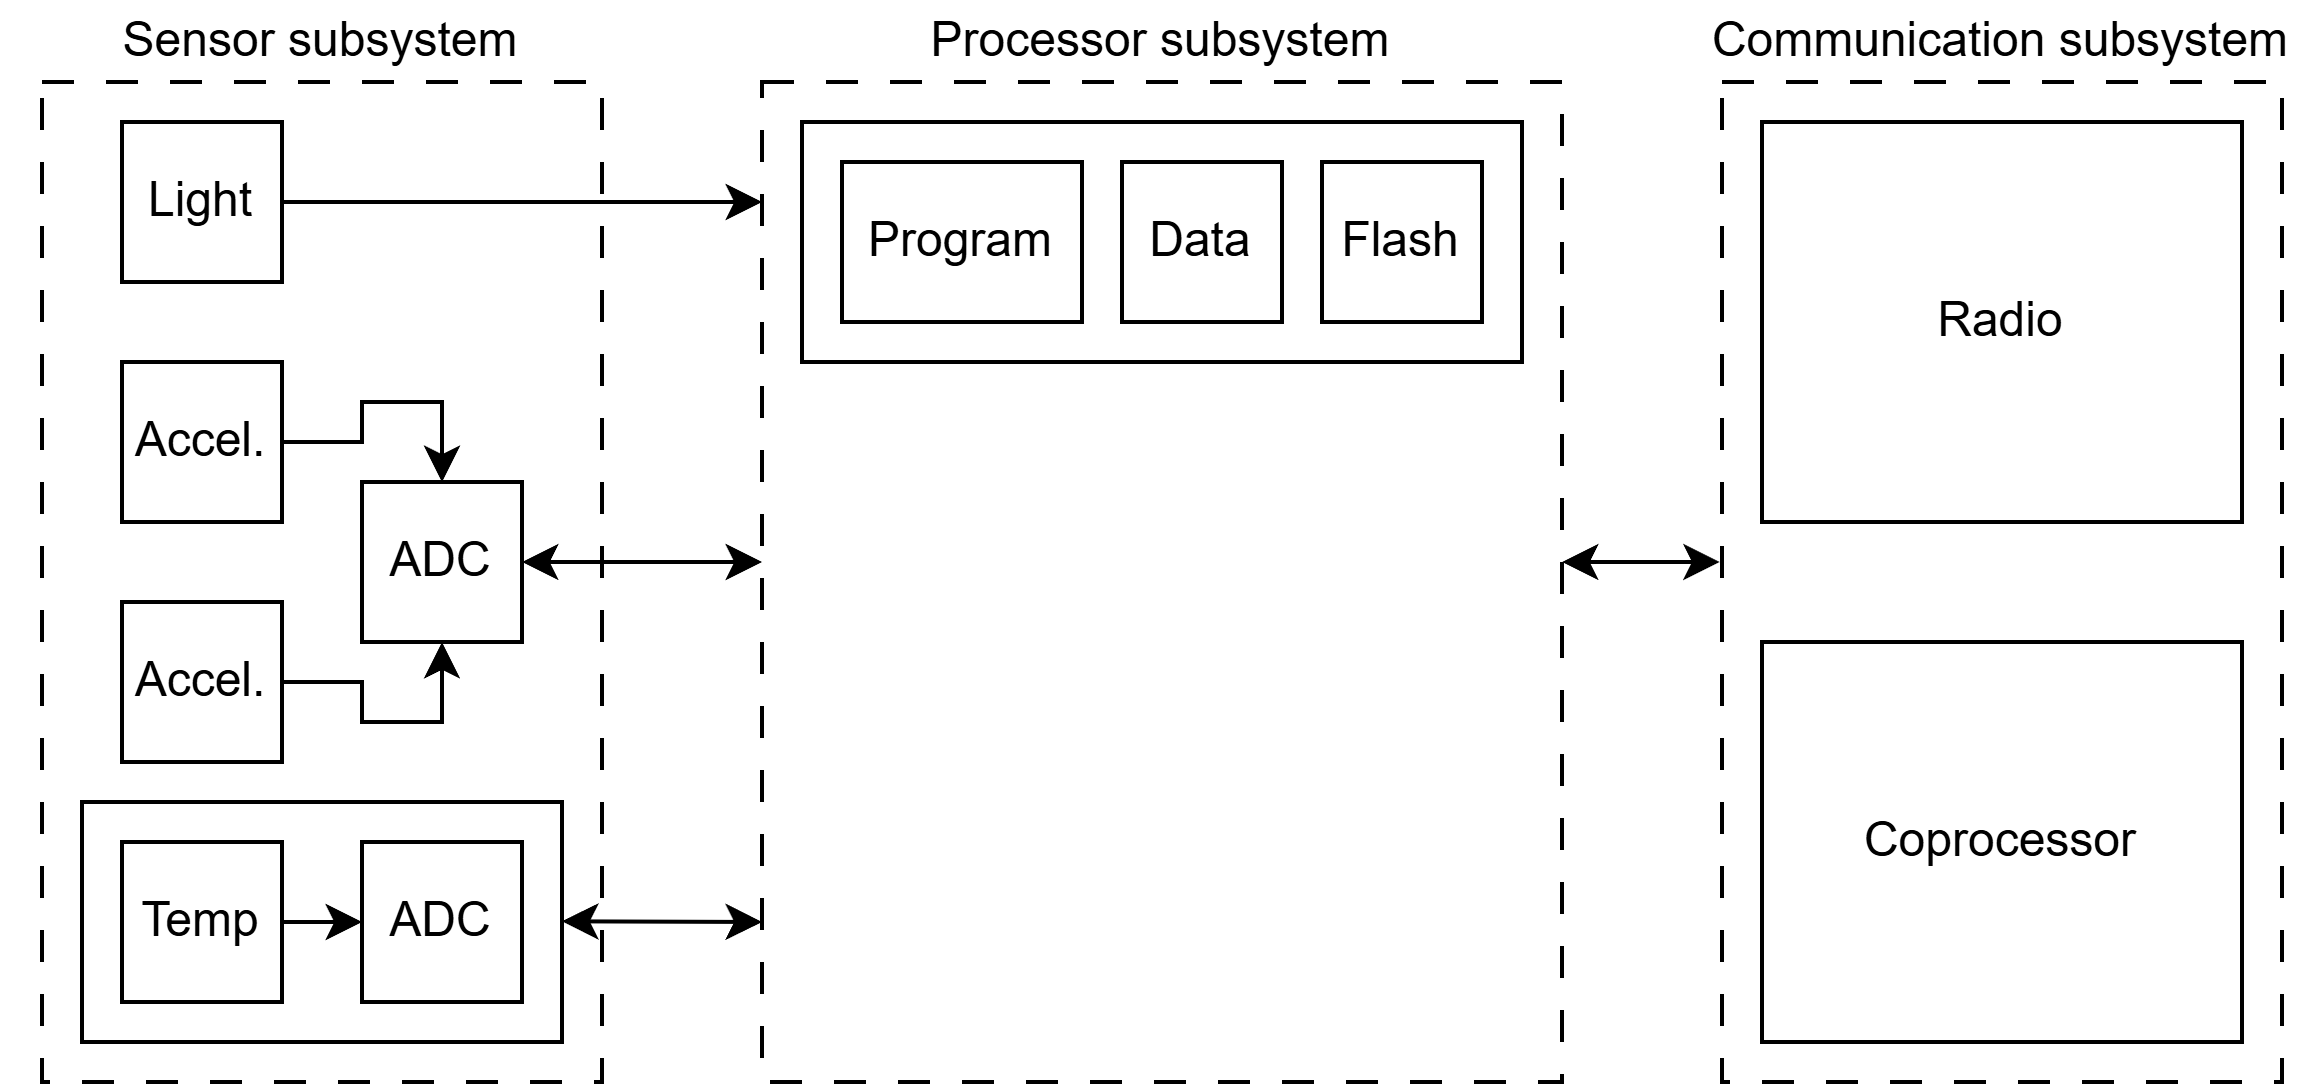
\includegraphics[width=0.75\linewidth]{images/sn.png}
    \caption{Sensor node architecture}
\end{figure}

\begin{definition}[\textit{Actuator}]
    An actuator is a device capable of acting on processes in order to modify conditions based on the input data.
\end{definition}

\subsection{Processor}
The processor subsystem of a sensor node is often designed based on the SHARC architecture. 
\begin{figure}[H]
    \centering
    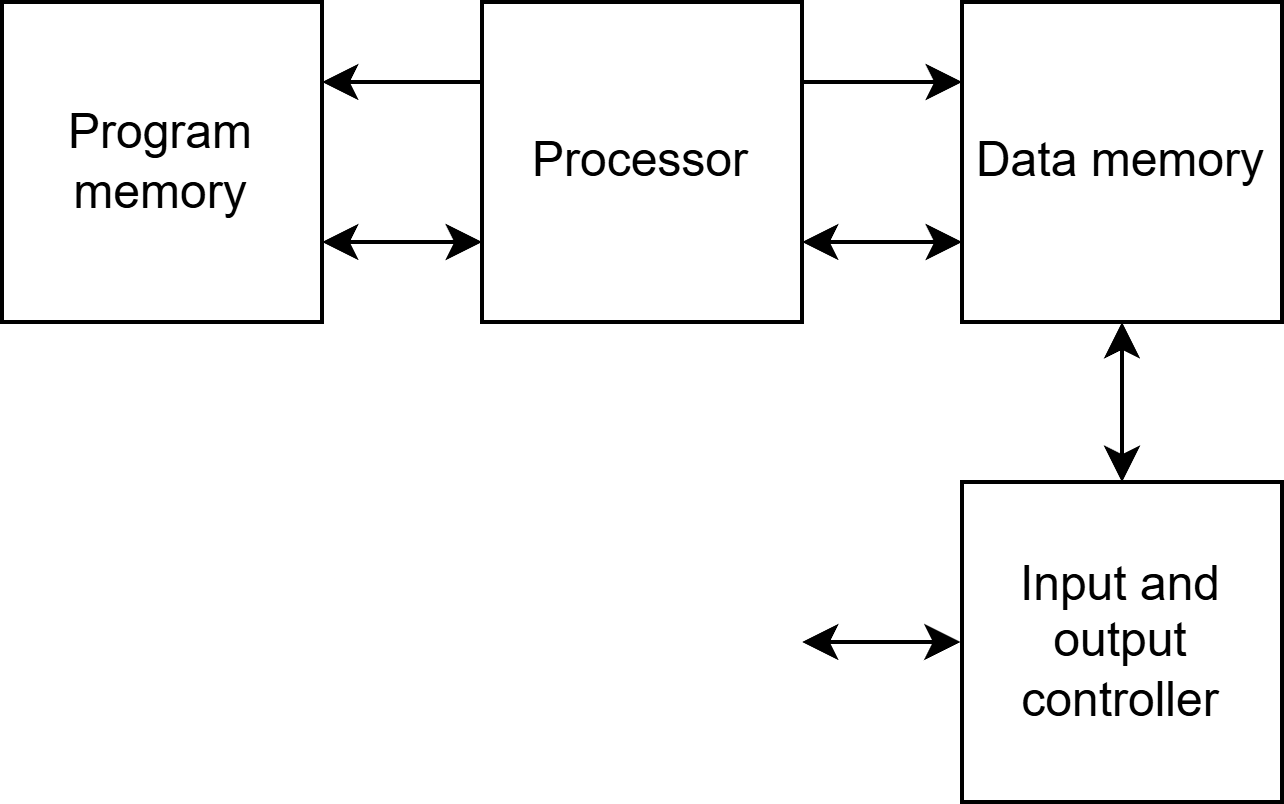
\includegraphics[width=0.5\linewidth]{images/pss.png}
    \caption{Processor SHARC architecture}
\end{figure}

A microcontroller is generally used as the processor in sensor nodes.
\begin{definition}[\textit{Microcontroller}]
    A microcontroller is a single integrated circuit designed for a specific application.
\end{definition}
\noindent A microcontroller is usually compose by a Central Processing Unit and a clock generator. 
It is usually equipped with RAM, flash memory and an EEPROM. 
It is connected with a serial BUS, I/O interfaces and analogic and digital converters. 
While microcontrollers are flexible and low-cost, they can compromise speed in certain use cases.

\begin{definition}[\textit{Digital Signal Processor}]
    A Digital Signal Processor is a specialized microprocessor optimized for processing discrete signals using digital filters.
\end{definition}
\noindent Digital Signal Processors excel at performing complex mathematical operations with extremely high efficiency. 
While they are well-suited for data-intensive operations, they are less flexible than microcontrollers.

\begin{definition}[\textit{Application Specific Integrated Circuit}]
    An Application Specific Integrated Circuit is a custom integrated circuit tailored for a specific application.
\end{definition}
\noindent Application Specific Integrated Circuits offer high speed and can be tailored for specific tasks, but they come with high development costs and limited flexibility once designed.

\begin{definition}[\textit{Field Programmable Gate Array}]
    A Field Programmable Gate Array has a high level architecture that allows for some degree of reconfigurability after manufacturing.
\end{definition}
\noindent Field Programmable Gate Arrays offer high-speed performance, supporting parallel programming, and moderate reconfigurability. 
However, they are more complex and costly than microcontrollers or Digital Signal Processors.

\subsection{Sensor}
Sensors samples the data from the real worlds and traduce them in digital format
\begin{figure}[H]
    \centering
    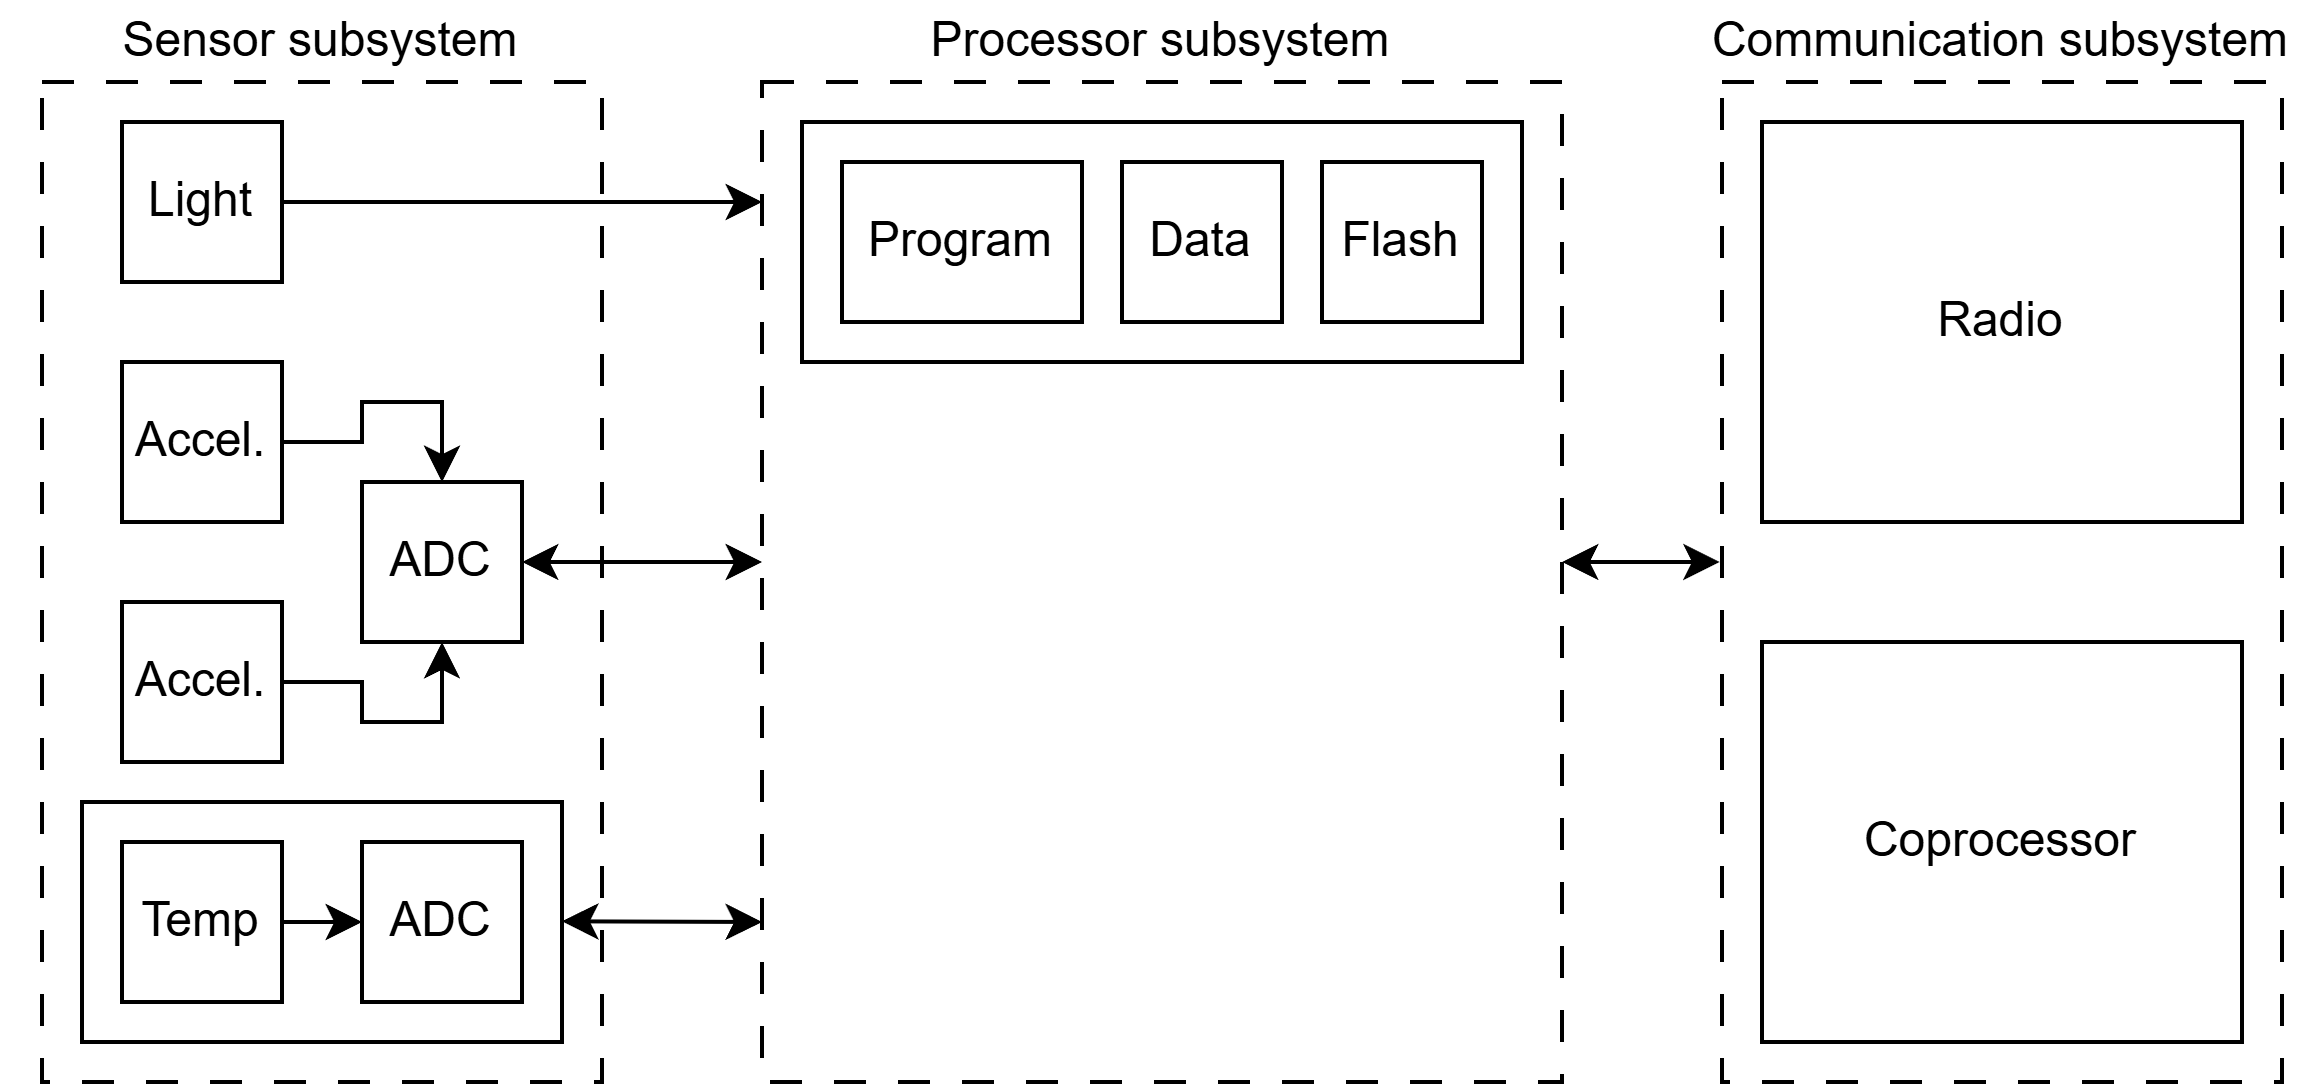
\includegraphics[width=0.75\linewidth]{images/iot2.png}
    \caption{Analog to digital converter}
\end{figure}

The Nyquist analog to digital converter involves reading a time-continuous signal at specific points in time. 
The sampling rate, or bandwidth, is the inverse of the sampling interval:
\[f_s=\dfrac{1}{T}\]
\noindent The key idea is that if the sampling frequency is properly set, the original signal can be losslessly reconstructed from its samples.
\begin{theorem}[Nyquist theorem]
    Given the signal bandwith $B$, we have that the sampling frequency must be chosen as:
    \[f_s=2B\]
\end{theorem}

Quantization is used to approximate the input voltage $V_{\text{in}}$ in a digital codeword. 
An ideal quantizer maps input to output with the smallest variation in the input causing a change in the codeword.
\begin{figure}[H]
    \centering
    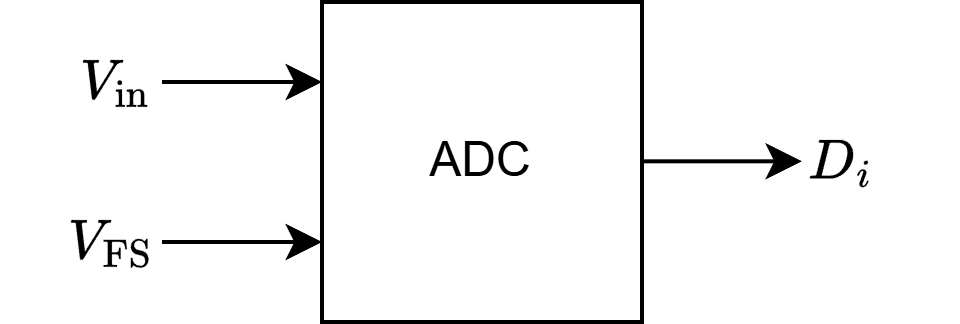
\includegraphics[width=0.5\linewidth]{images/quant.png}
    \caption{Quantization}
\end{figure}
\noindent The resolution refers to the smallest input variation that causes a change in the codeword:
\[\text{LBS}=\dfrac{V_{\text{FS}}}{2^n}\]
Here, $V_{\text{FS}}$ is the full-scale voltage and $n$ is the number of bits of resolution.
The quantization error occurs when the output voltage either overestimates or underestimates the input voltage. 
This error decreases as the resolution increases.

\subsection{Power consumption}
The absence of cables in wireless sensors and actuators means no wired power or connectivity. 
A sensor node typically operates with a limited power source, and its lifetime directly depends on the battery lifetime. 
The goal is to maximize the energy provided while minimizing the cost, volume, weight, and recharge requirements.
There are two main types of batteries used:
\begin{itemize}
    \item Primary batteries, which are not rechargeable.
    \item Secondary batteries, which are rechargeable, but only make sense when paired with some form of energy harvesting.
\end{itemize}

\paragraph*{Power cycle}
The power cycle of an Internet of Things device consists of sleep and active states (wake-up and work). 
During the sleep state, power consumption is minimal, with only essential components running.
\begin{figure}[H]
    \centering
    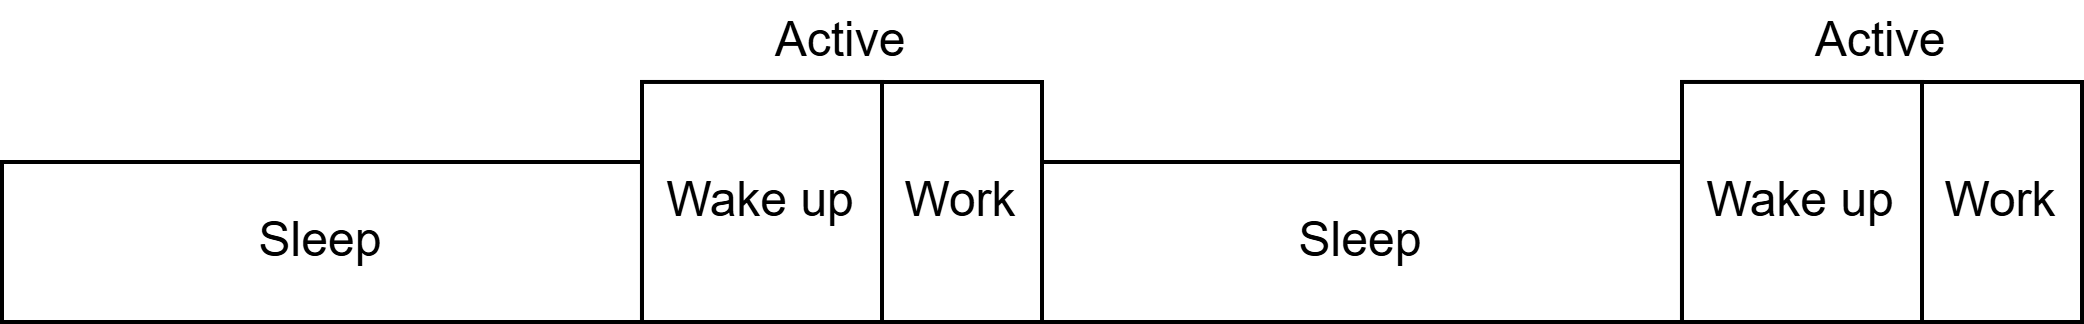
\includegraphics[width=0.75\linewidth]{images/iot3.png}
    \caption{Internet of Things device life cycle}
\end{figure}
\noindent The average power consumption is then defined as:
\[P_{\text{avg}}=f_{\text{sleep}}P_{\text{sleep}}+f_{\text{wakeup}}P_{\text{wakeup}}+f_{\text{work}}P_{\text{work}}\]
Here, $f_{\text{sleep}}$, $f_{\text{wakeup}}$, and $f_{\text{work}}$ are the fractions of time spent in sleep, wake-up, and work states, respectively.
Then, the lifetime of the device is given by:
\[\text{lifetime}=\dfrac{\text{energy stored}}{P_{\text{avg}}-P_{\text{gen}}}\]
Here, $P_{\text{gen}}$ is the power generated.

\subsubsection{Data transmission}
When data needs to be sent, the device first wakes up and then performs the actual transmission. 
The total energy consumption for this process is given by:
\[E_\text{tx}=P_\text{tx}(T_\text{wu}+T_\text{tx})+P_0T_{tx}\]
\noindent Here, $P_{tx}$ is the power consumed by the transmitter, $P_0$ is the output power of the transmitter, $T_{tx}$ is the time taken to transmit a packet, and $T_{wu}$ is the wake-up time.

\subsubsection{Data reception}
When the device needs to receive data, it first wakes up and then performs the reception. 
The total energy consumption in this case is:
\[E_\text{tx}=P_\text{rx}(T_\text{uw}+T_\text{rx})\]
Here, $P_{rx}$ is the power consumed by the receiver, $T_{rx}$ is the time taken to receive a packet, and $T_{wu}$ is the wake-up time.

\paragraph*{Sensitivity}
Each receiver is characterized by a sensitivity parameter, which is the minimum input signal power required for the receiver to demodulate the data correctly. 
Knowing this sensitivity, the required emitted power at the transmitter can be determined by inverting the propagation law of the communication channel.

\subsubsection{Emitted power}
The emitted power is often a tunable parameter, and it is generally considered good practice to set it to the lowest value that still allows for reliable reception. 
The quality of the reception process is typically measured using metrics like:
\begin{itemize}
    \item \textit{Bit Error Rate}: the fraction of bits that are incorrectly received. 
    \item \textit{Packet Error Rate}: the fraction of packets that are not received correctly.
\end{itemize}
The relationship between $\text{BER}$ and $\text{PER}$, for a packet of length $l$ with independent errors, is given by:
\[\text{PER}=1-(1-\text{BER})^l\]
Both $\text{BER}$ and $\text{PER}$ are influenced by the level of noise in the transmission and reception channels, which in turn is determined by the transmitted and received power. 
The Signal-to-Interference-plus-Noise Ratio is a key factor in determining this quality, and is calculated as:
\[\text{SINR}=10\log\left(\dfrac{P_{\text{recv}}}{N_0+\sum_{i=1}^{k}I_i}\right)\]
Here, $N_0$ is the thermal noise (KTB), $P_{\text{recv}}$ is the received power, and $I_i$ are the interference contributions from other signals.
Given the SINR and the specific modulation of the channel, $\text{BER}$ can be computed.

\subsubsection{Processing power}
The power dissipation of the CPU is due to several factors, including:
\[P_{\text{p}}=P_{\text{dyn}}+P_{\text{sc}}+P_{\text{leak}}\]
Here, $P_{\text{dyn}}=CfV^2$ is the power consumed by the work done, $P_{\text{sc}}$ is the power lost due to short circuits, and $P_{\text{leak}}$ is the power lost due to leakage.
Local data processing is crucial in minimizing power consumption, especially in multi-hop networks.

\subsubsection{Sensor power}
The power consumption due to sensing is highly dependent on the type of sensor used. 
A rough model for the power consumption of an analog to digital converter can be expressed as:
\[P_s\approx f_s2^n\]
\noindent Here, $f_s$ is the sampling frequency, and $n$ is the resolution of the analog to digital converter in bits.